% !TEX root = main.tex
\section{Results and findings}
We will now present the results of our experiments, going through each one of the already presented measures.

\subsection{Regularity}
As we stated before, the regularity tells us whether the users tend to be regular while tapping the red balloon during the activity. Let us first consider the first one, \testfirst. In Figure~\ref{fig:reg1} we can see the plot of the means squared error (from now on referred as MSE) for the activity. As we can see some sessions are very irregular in the beginning but all of them tend to a very low MSE, meaning that all the users are becoming very regular after a few seconds of activity. Besides of the observation of the graph this result is also confirmed by a very low average MSE of 0.15.

\todo[inline]{Unit measures on graphs. Also remove or mark the average line.}

\begin{figure}[h!t]
\centering
	{\setlength{\fboxsep}{1.5pt}
	 \fbox{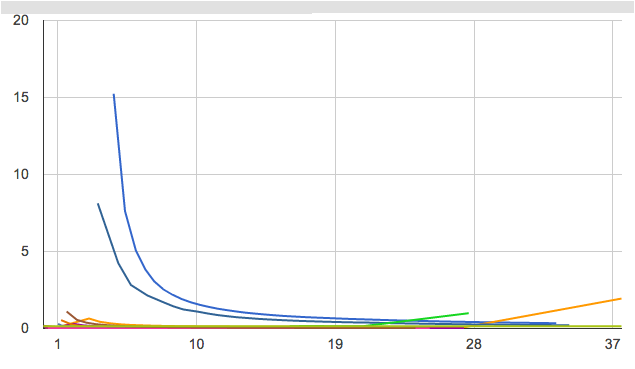
\includegraphics[width=0.45\textwidth]{reg1}}}
\caption{Regularity of \testfirst experiment}
\label{fig:reg1}
\end{figure}

On the other hand the MSE for the \testsecond experiment is very irregular, as shown in Figure~\ref{fig:reg2}, and does not tend to zero as the first one. We can observe that approximately for 5 seconds most of the users tend to tap regularly on the balloon, becoming then very irregular later on. This is probably due to the fact that during the first seconds of the activity they are trying to understand the balloon's behavior and when they get it they trying to inflate it as fast as they can, constantly increasing their tapping speed. This leads to very irregular tap intervals and a higher average MSE of 1.78.

\begin{figure}[h!t]
\centering
	{\setlength{\fboxsep}{1.5pt}
	 \fbox{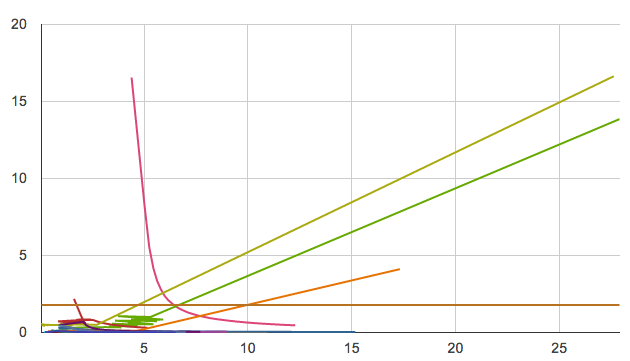
\includegraphics[width=0.45\textwidth]{reg2}}}
\caption{Regularity of \testsecond experiment}
\label{fig:reg2}
\end{figure}